
\subsection*{1.}

\begin{center}
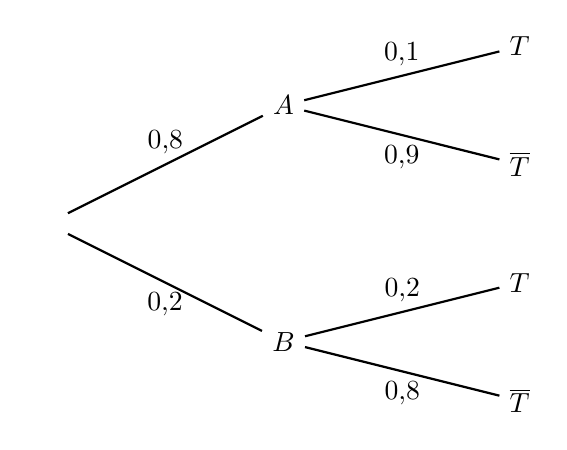
\begin{tikzpicture}[thick, scale=1.5]
\node (P_-1_0) at (-2,-1.5) {$\phantom{A}$};
\node (P_0_0) at (0,-0.5) {$A$};
\draw (P_-1_0) -- (P_0_0) node[midway, above] {$0{,}8$};
\node (P_1_0) at (2,-0) {$T$};
\draw (P_0_0) -- (P_1_0) node[midway, above] {$0{,}1$};
\node (P_1_1) at (2,-1) {$\overline{T}$};
\draw (P_0_0) -- (P_1_1) node[midway, below] {$0{,}9$};
\node (P_0_2) at (0,-2.5) {$B$};
\draw (P_-1_0) -- (P_0_2) node[midway, below] {$0{,}2$};
\node (P_1_2) at (2,-2) {$T$};
\draw (P_0_2) -- (P_1_2) node[midway, above] {$0{,}2$};
\node (P_1_3) at (2,-3) {$\overline{T}$};
\draw (P_0_2) -- (P_1_3) node[midway, below] {$0{,}8$};
\end{tikzpicture}
\end{center}

\subsection*{2.}

On a \( P(A \cap T) = P(A) \times P_A(T) = 0{,}8 \times 0{,}1 = 0{,}08 \), soit 8 \%.

\subsection*{3.}

\( B \cap \overline{T} \) désigne l'événement « la boîte prélevée provient du fournisseur \(\textit{Bon Thé}\) et ne contient pas de traces de pesticides ».

\[
P(B \cap \overline{T}) = P(B) \times P_B(\overline{T}) = 0{,}2 \times 0{,}8 = 0{,}16, \text{ soit 16 \%}.
\]

\subsection*{4.}

On a, de la même façon qu'à la question précédente :
\[
P(A \cap \overline{T}) = P(A) \times P_A(\overline{T}) = 0{,}8 \times 0{,}9 = 0{,}72, \text{ soit 72 \%}.
\]
D'après la loi des probabilités totales :
\[
P(\overline{T}) = P(A \cap \overline{T}) + P(B \cap \overline{T}) = 0{,}72 + 0{,}16 = 0{,}88, \text{ soit 88 \%}.
\]

\subsection*{5.}

\begin{itemize}
    \item On a \( P(T) = 1 - P(\overline{T}) = 1 - 0{,}88 = 0{,}12 \).
    \item On a \( P(B \cap T) = P(B) \times P_B(T) = 0{,}2 \times 0{,}2 = 0{,}04 \).
\end{itemize}

Il faut donc trouver :
\begin{align*}
P_T(B) &= \dfrac{P(T \cap B)}{P(T)} \\
&= \dfrac{P(B \cap T)}{P(T)} \\
&= \dfrac{0{,}04}{0{,}12} \\
&= \dfrac{4}{12} \\
&= \dfrac{1}{3} \approx 0{,}33.
\end{align*}
Si une boîte a des traces de pesticides il y a deux chances sur trois qu'elle provienne de \textit{Au bon thé} et une chance sur trois qu'elle provienne de \textit{Bon thé}.


